\scanpage{151}\mspage{6}
\unsure{groupe|groupes} \unsure{formel|formels} est concentré en les groupes formels commutatifs, découvert semble-t-il par Dieudonné \dots). La question que je voudrais soulever est la généralisation aux groupes dans $(n\text{-cat})$, on s'attend à trouver des complexes de chaines non comm
\diagram{\begin{tikzcd}[ampersand replacement=\&,column sep=small]
L_n\arrow[r,no head,to path={-- (\tikztotarget) -- ++(0.025,0.055)}] \& L_{n-\unsure{,|1}}\arrow[r,no head,to path={-- (\tikztotarget) -- ++(0.025,0.055)}] \& \ldots\arrow[r,no head,to path={-- (\tikztotarget) -- ++(0.025,0.055)}] \& L_1\arrow[r,no head,to path={-- (\tikztotarget) -- ++(0.025,0.055)}] \& L_0\arrow[r] \& 1
\end{tikzcd}}
avec des structures supplémentaires sans doute du type $\unsure{\Theta|\theta}$, mais lesquelles ? Il est entendu que la signification topologique de ces structures, c'est qu'elles expriment exactement les ``types d'homotopie tronqués en dim $\leq n$'' des groupes topologiques. \inserted{\unsure{ou encore} les types d'hom \unsure{tronqués|tr.\ \deleted{qués}} en dim $\leq n+1$ des espaces top \unsure{ponctues|ponctués} connexes \dots)} \unsure{.} As-tu des \unsure{candïdats|candidats} à proposer ?
% Interlinear insertion guide. The left end is in the gap before As-tu;
% the long horizontal part runs below the end of the added line.
\figure{\begin{tikzpicture}[x=1cm,y=1cm]
\draw (0,-0.42) .. controls (-0.035,-0.22) and (-0.07,-0.08) .. (0.10,0.02)
.. controls (0.30,0.11) and (1.25,0.07) .. (1.72,0.06)
.. controls (2.38,0.035) and (3.06,0.055) .. (3.33,0.10)
-- (3.34,0.20);
\end{tikzpicture}}

\figure{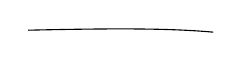
\begin{tikzpicture}\draw (0,0) .. controls (1.1,0.025) and (1.8,0.025) .. (2.35,-0.025);\end{tikzpicture}}

\unsure{.} Tes réflexions de bidualité \inserted{et d'homologie}, pour formelles qu'elles soient, se rattachent à une foule de développements, dont certains seulement existent\unsure{,} dès à présent, et d'autres demanderaient des développements considérables. Voici les réminiscences que m'ouvrent tes \unsure{noïves|naïves|noires} questions :
% Guide below et d'homologie; its left leg descends to the gap
% after bidualité, before the comma/pour portion of the baseline.
\figure{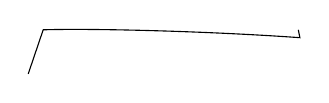
\begin{tikzpicture}[x=1cm,y=1cm]
\draw (0,-0.46) -- (0.19,0.10)
.. controls (0.84,0.12) and (2.33,0.08) .. (3.45,0.00)
-- (3.43,0.10);
\end{tikzpicture}}
% archive sheet number: 151
